% Standalone figure: Fig. 1 method-overview schematic -- the coverage-debt
% audit pipeline. Symbolic only (no data plotted); box terminology matches
% paper_isprs.tex \S\ref{sec:methods}, \S\ref{sec:reportcard},
% \S\ref{sec:limitations} (frozen GFM encoder, spatial-Mondrian,
% coverage-debt report card; no universal restoration vs conditional
% labeled-target recalibration).
% Compile: make  (or: latexmk -pdf fig0_overview.tex)
%
% 2026-08-12 beautify: horizontal five-stage flow + centered outcome fork
% (fills column width; short vertical footprint for float placement). Icons
% sit inside stage cards with Okabe-Ito accent bars; outcome color is
% border/fill only (in-figure text stays black).
% 2026-08-12 leak fix: plain-English outcome labels (no gate jargon).
\documentclass[border=2pt]{standalone}
\usepackage[T1]{fontenc}
\usepackage{tikz}
\usetikzlibrary{arrows.meta,calc,positioning,fit}

% Colorblind-safe Okabe-Ito (matches ../figures/ggtheme.R).
\definecolor{cPipe}{HTML}{0072B2}    % blue: pipeline
\definecolor{cCalib}{HTML}{56B4E9}   % sky: calibration / report accent
\definecolor{cFail}{HTML}{D55E00}    % vermillion: no universal restoration
\definecolor{cCond}{HTML}{009E73}    % bluish green: conditional recalibration
\definecolor{cInk}{HTML}{1A1A1A}
\definecolor{cMute}{HTML}{595959}
\definecolor{cLine}{HTML}{B8B8B8}
\definecolor{cSurface}{HTML}{FAFAFA}
\definecolor{cAccentSoft}{HTML}{E8F3FA}

\begin{document}
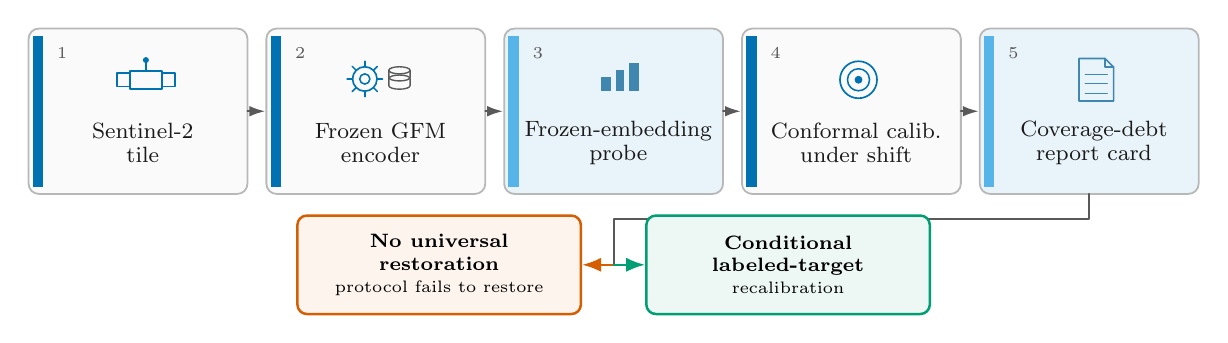
\begin{tikzpicture}[
  x=1mm, y=1mm,
  font=\rmfamily\fontsize{7.8}{9.0}\selectfont,
  line cap=round, line join=round,
  >=Latex,
  flow/.style={draw=cMute, line width=0.7pt,
    -{Latex[length=2.0mm,width=1.35mm]}, shorten >=0.15mm},
  stage/.style={draw=cLine, line width=0.65pt, rounded corners=1.3mm,
    fill=cSurface, minimum width=27.8mm, minimum height=21.0mm,
    inner sep=0pt, outer sep=0pt, align=center},
  stageAccent/.style={stage, fill=cAccentSoft},
  outbox/.style={draw, line width=0.9pt, rounded corners=1.2mm,
    align=center, minimum width=36mm, minimum height=12.5mm,
    inner sep=1.4mm, font=\rmfamily\fontsize{7.2}{8.4}\selectfont},
  steplab/.style={font=\rmfamily\fontsize{6.4}{7.2}\selectfont, text=cMute},
  titlelab/.style={font=\rmfamily\fontsize{7.7}{8.8}\selectfont, text=cInk},
  sublab/.style={font=\rmfamily\fontsize{6.4}{7.4}\selectfont, text=cMute},
]

% ---- Accent bar (left strip inside a named stage node) ----
\newcommand{\accentbar}[2]{%
  \fill[#2] ([xshift=0.55mm,yshift=-0.9mm]#1.north west)
    rectangle ([xshift=1.85mm,yshift=0.9mm]#1.south west);}

% ---- Stage cards (left → right) ----
\node[stage] (tile) at (0,0) {};
\accentbar{tile}{cPipe}
\node[steplab, anchor=north west] at ($(tile.north west)+(2.4mm,-1.2mm)$) {1};
\node[titlelab, align=center] at ($(tile.center)+(0.6mm,-4.0)$)
  {Sentinel-2\\tile};

\node[stage, right=2.4mm of tile] (enc) {};
\accentbar{enc}{cPipe}
\node[steplab, anchor=north west] at ($(enc.north west)+(2.4mm,-1.2mm)$) {2};
\node[titlelab, align=center] at ($(enc.center)+(0.6mm,-4.0)$)
  {Frozen GFM\\encoder};

\node[stageAccent, right=2.4mm of enc] (probe) {};
\accentbar{probe}{cCalib}
\node[steplab, anchor=north west] at ($(probe.north west)+(2.4mm,-1.2mm)$) {3};
\node[titlelab, align=center] at ($(probe.center)+(0.6mm,-4.0)$)
  {Frozen-embedding\\probe};

\node[stage, right=2.4mm of probe] (calib) {};
\accentbar{calib}{cPipe}
\node[steplab, anchor=north west] at ($(calib.north west)+(2.4mm,-1.2mm)$) {4};
\node[titlelab, align=center] at ($(calib.center)+(0.6mm,-4.0)$)
  {Conformal calib.\\under shift};

\node[stageAccent, right=2.4mm of calib] (report) {};
\accentbar{report}{cCalib}
\node[steplab, anchor=north west] at ($(report.north west)+(2.4mm,-1.2mm)$) {5};
\node[titlelab, align=center] at ($(report.center)+(0.6mm,-4.0)$)
  {Coverage-debt\\report card};

% ---- Icons (above labels, inside each card) ----
% 1. Satellite tile
\begin{scope}[shift={($(tile.center)+(1.0mm,4.0mm)$)}, thick, cPipe]
  \draw[line width=0.65pt] (-2.0mm,-1.15mm) rectangle (2.0mm,1.15mm);
  \draw[line width=0.55pt] (-3.7mm,-0.85mm) rectangle (-2.0mm,0.85mm);
  \draw[line width=0.55pt] (2.0mm,-0.85mm) rectangle (3.7mm,0.85mm);
  \draw[line width=0.55pt] (0,1.15mm) -- (0,2.5mm);
  \fill (0,2.5mm) circle (0.38mm);
\end{scope}

% 2. Gear + stacked cylinders (interchangeable frozen backbones)
\begin{scope}[shift={($(enc.center)+(-1.4mm,4.1mm)$)}, thick, cPipe]
  \draw[line width=0.6pt] (0,0) circle (1.55mm);
  \foreach \a in {0,45,...,315}{\draw[line width=0.55pt] (\a:1.55mm) -- (\a:2.25mm);}
  \fill[cSurface] (0,0) circle (0.65mm);
  \draw[line width=0.55pt] (0,0) circle (0.65mm);
\end{scope}
\begin{scope}[shift={($(enc.center)+(3.0mm,3.7mm)$)}, thick, cMute]
  \foreach \dy in {0,1.05mm}{
    \draw[line width=0.5pt]
      (-1.35mm,0.45mm+\dy) -- (-1.35mm,-0.45mm+\dy)
      arc (180:360:1.35mm and 0.45mm)
      -- (1.35mm,0.45mm+\dy)
      arc (0:180:1.35mm and 0.45mm);
  }
  \draw[line width=0.5pt] (-1.35mm,0.45mm+1.05mm) arc (180:360:1.35mm and 0.45mm);
\end{scope}

% 3. Embedding bars
\begin{scope}[shift={($(probe.center)+(0.8mm,2.6mm)$)}, cCalib!75!black]
  \fill (-2.4mm,0) rectangle (-1.15mm,1.7mm);
  \fill (-0.55mm,0) rectangle (0.55mm,2.6mm);
  \fill (1.15mm,0) rectangle (2.4mm,3.5mm);
\end{scope}

% 4. Calibration bullseye
\begin{scope}[shift={($(calib.center)+(0.9mm,4.0mm)$)}, thick, cPipe]
  \draw[line width=0.6pt] (0,0) circle (2.35mm);
  \draw[line width=0.55pt] (0,0) circle (1.4mm);
  \fill (0,0) circle (0.5mm);
\end{scope}

% 5. Report-card document
\begin{scope}[shift={($(report.center)+(0.9mm,4.0mm)$)}, thick, cCalib!75!black]
  \draw[line width=0.6pt]
    (-2.2mm,-2.7mm) -- (-2.2mm,2.7mm) -- (1.1mm,2.7mm) --
    (2.2mm,1.6mm) -- (2.2mm,-2.7mm) -- cycle;
  \draw[line width=0.55pt] (1.1mm,2.7mm) -- (1.1mm,1.6mm) -- (2.2mm,1.6mm);
  \foreach \y in {0.7mm,-0.5mm,-1.7mm}{
    \draw[line width=0.45pt] (-1.4mm,\y) -- (1.4mm,\y);
  }
\end{scope}

% ---- Flow arrows ----
\draw[flow] (tile.east) -- (enc.west);
\draw[flow] (enc.east) -- (probe.west);
\draw[flow] (probe.east) -- (calib.west);
\draw[flow] (calib.east) -- (report.west);

% ---- Outcome fork (centered under full pipeline) ----
\coordinate (mid) at ($(tile.south)!0.5!(report.south)$);
\coordinate (drop) at ($(report.south)+(0,-3.2mm)$);
\coordinate (branch) at ($(mid)+(0,-9.0mm)$);

\draw[cMute, line width=0.7pt] (report.south) -- (drop) -| (branch);

\node[outbox, draw=cFail, fill=cFail!7, left=4.0mm of branch] (fail)
  {\textbf{No universal}\\[-0.1mm]\textbf{restoration}\\[-0.15mm]
   {\fontsize{6.0}{6.8}\selectfont protocol fails to restore}};
\node[outbox, draw=cCond, fill=cCond!7, right=4.0mm of branch] (cond)
  {\textbf{Conditional}\\[-0.1mm]\textbf{labeled-target}\\[-0.15mm]
   {\fontsize{6.0}{6.8}\selectfont recalibration}};

\draw[->, cFail, line width=0.85pt] (branch) -- (fail.east);
\draw[->, cCond, line width=0.85pt] (branch) -- (cond.west);

\end{tikzpicture}
\end{document}
